% ============================================================================
% CAPÍTULO 4 — METODOLOGIA
% ============================================================================

\chapter{Metodologia}
\label{cap:metodologia}

Nesta seção, é apresentado o plano metodológico para o desenvolvimento do pipeline de montagem de mitogenomas. A abordagem combina etapas de análise bioinformática com práticas consolidadas de engenharia de software, seguindo um processo de desenvolvimento sistemático descrito na seção 4.1, antes de detalhar a arquitetura do pipeline e suas etapas constituintes.

\section{Processo de Desenvolvimento de Software}

O desenvolvimento do pipeline seguiu uma abordagem de \textbf{desenvolvimento iterativo e incremental}, metodologia consolidada na engenharia de software em que o sistema é construído em ciclos sucessivos, cada um produzindo uma versão funcional e testável do produto \cite{larman2003}. Essa abordagem se contrapõe ao modelo cascata (\textit{waterfall}), no qual todas as fases --- levantamento de requisitos, projeto, implementação e teste --- são executadas sequencialmente e o produto só é validado ao final. No contexto de software científico, em que os requisitos frequentemente evoluem à medida que os resultados são analisados, o modelo iterativo é amplamente recomendado \cite{wilson2014}.

O ciclo de desenvolvimento foi organizado em duas fases principais, cada uma constituindo uma iteração completa com entrega funcional:

\begin{itemize}
    \item \textbf{Fase 1 --- Montagem}: implementação dos módulos de download (SRA-Toolkit), controle de qualidade (FastQC, Trim Galore) e montagem (NOVOPlasty), com containerização em Docker e orquestração via Nextflow. Ao final desta fase, o pipeline já era capaz de produzir mitogenomas completos e circularizados a partir de um acesso SRA.
    \item \textbf{Fase 2 --- Anotação e entregáveis}: adição dos módulos de análise piloto de qualidade (Pilot QC), anotação funcional (MITOS2), geração de estruturas secundárias de RNA (ViennaRNA/RNAplot), produção de arquivos para submissão ao GenBank (GenBank Flat File) e compilação automática de entregáveis.
\end{itemize}

Cada fase produziu um pipeline funcional e independente. A Fase 1 foi preservada como branch separada no repositório Git (\texttt{fase1-montagem}), permitindo uso e validação independente por terceiros --- uma prática de versionamento semântico que garante rastreabilidade e facilita a manutenção \cite{sommerville2016}.

\begin{figure}[H]
    \centering
    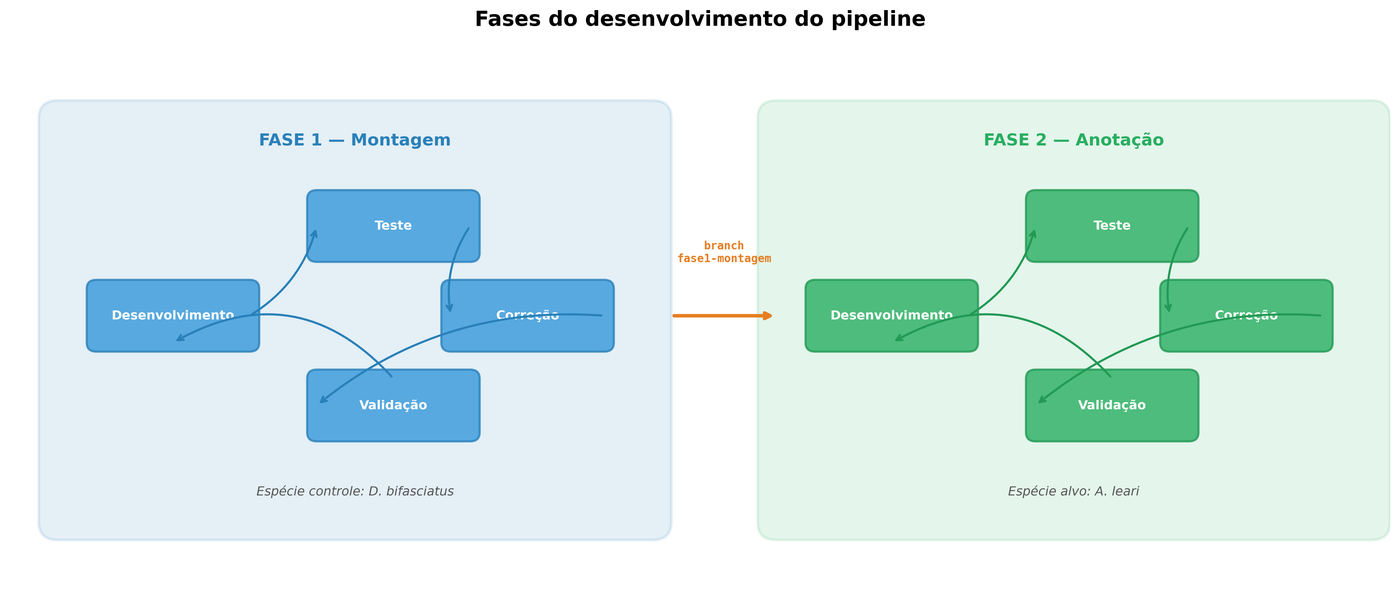
\includegraphics[width=0.85\textwidth]{imagens/fases_desenvolvimento.png}
    \caption{Diagrama de fases do desenvolvimento do pipeline: Fase 1 (Montagem) e Fase 2 (Anotação), com indicação dos ciclos iterativos e das espécies utilizadas em cada fase.}
    \label{fig:fases_desenvolvimento}
\end{figure}

\subsection{Validação por Espécie-Controle}

Um elemento central da estratégia de verificação e validação (V\&V) foi o emprego de uma \textbf{espécie-controle} com mitogenoma previamente depositado em banco de dados público. Antes de aplicar o pipeline à espécie-alvo (a arara-azul-de-lear), cuja sequência mitocondrial era inédita, o sistema foi integralmente validado com \textit{Diploprion bifasciatus}, cujo mitogenoma de referência (PZ143763.1) está depositado no GenBank. Essa estratégia permitiu comparar a montagem obtida pelo pipeline com a sequência de referência conhecida, verificando a correção funcional do sistema em condições controladas antes de aplicá-lo a dados sem referência prévia.

No desenvolvimento de software científico, a validação com dados de referência conhecida é considerada uma das práticas mais importantes para garantir a confiabilidade dos resultados computacionais \cite{wilson2014}. Essa abordagem é análoga ao conceito de \textit{oracle testing} na engenharia de software, em que uma fonte externa de verdade é utilizada para validar as saídas do sistema sob teste \cite{sommerville2016}.

\subsection{Tratamento de Erros e Correções Iterativas}

O modelo iterativo também se manifestou na resolução de problemas técnicos encontrados durante a execução do pipeline. Exemplos concretos incluem:

\begin{enumerate}
    \item \textbf{Incompatibilidade do SRA-Toolkit}: a descoberta de que o \texttt{fasterq-dump} do SRA-Toolkit 3.x não implementa o flag \texttt{-X} para limitação de leituras na origem, corrigida pela adoção de truncamento pós-conversão utilizando o utilitário \texttt{head};
    \item \textbf{Flag do RNAplot}: a incompatibilidade do flag \texttt{-{}-output-format=svg} na versão empacotada do ViennaRNA, corrigida para a sintaxe \texttt{-f svg} aceita pela versão instalada;
    \item \textbf{Frameshift do gene ND3}: a detecção, durante a análise dos resultados do MITOS2, de que o gene ND3 apresenta um frameshift biologicamente real e documentado em aves \cite{mindell1998}, levando à implementação de uma lógica de unificação (\texttt{join}) nos scripts de conversão para GenBank.
\end{enumerate}

Cada correção foi implementada, testada e integrada antes do avanço para a próxima etapa, em conformidade com o princípio de retroalimentação rápida (\textit{fail fast, fix immediately}) característico de metodologias ágeis \cite{sommerville2016}.

\subsection{Aderência às Boas Práticas de Computação Científica}

A adoção das práticas descritas acima situa este trabalho no contexto das boas práticas para computação científica sistematizadas por \citeonline{wilson2014}, que recomendam:

\begin{enumerate}
    \item \textbf{Controle de versão} para todo código-fonte --- implementado via Git com histórico completo de commits descritivos e branches para marcos significativos;
    \item \textbf{Automação de tarefas repetitivas} --- implementada via Nextflow, que orquestra todas as etapas sem intervenção manual;
    \item \textbf{Testes com dados conhecidos} --- implementados pela validação com espécie-controle (\textit{D.~bifasciatus});
    \item \textbf{Registro de dependências e ambientes} --- implementado via Dockerfiles com versões explicitamente fixadas para todas as ferramentas;
    \item \textbf{Documentação do propósito e das decisões de design} --- implementada no repositório (README, guia de execução) e neste documento.
\end{enumerate}

Essa abordagem metodológica não é apenas uma decisão de conveniência, mas uma necessidade reconhecida na literatura: estudos demonstram que a falta de práticas formais de engenharia de software em projetos científicos é uma das principais causas de irreprodutibilidade computacional \cite{baker2016,peng2011}.

\section{Visão Geral do Pipeline}

O pipeline proposto neste trabalho foi concebido para realizar a montagem e anotação de genomas mitocondriais a partir de dados de sequenciamento de nova geração (NGS), integrando ferramentas bioinformáticas consolidadas em um ambiente de execução automatizado, reprodutível e portável. A arquitetura segue uma estrutura modular, em que cada etapa corresponde a uma fase distinta do processamento dos dados, sendo encapsulada em containers Docker para garantir consistência na execução \cite{merkel2014} e integrada por meio do gerenciador de workflows Nextflow \cite{ditommaso2017}.

De forma geral, o pipeline é composto por sete macroetapas principais, organizadas em uma cadeia de redução progressiva de dados que transforma dezenas de gigabytes de leituras brutas em um mitogenoma anotado de $\sim$17~KB --- viabilizando a execução em computadores pessoais sem necessidade de servidores. A primeira é a \textbf{análise piloto de qualidade (Pilot QC)}, um estágio opcional que analisa automaticamente uma subamostra dos dados para determinar o volume ideal de leituras a serem processadas, evitando downloads desnecessários em datasets grandes. A segunda etapa é a \textbf{aquisição e preparo dos dados}, responsável por obter datasets públicos em repositórios como o Sequence Read Archive (SRA) do NCBI \cite{leinonen2011}. Em seguida, realiza-se o \textbf{controle de qualidade e pré-processamento}, que envolve a avaliação das leituras por meio do FastQC \cite{andrews2010} e a remoção de adaptadores e bases de baixa qualidade utilizando o Trim Galore \cite{babraham2019}, que por sua vez utiliza o Cutadapt \cite{martin2011} internamente.

A quarta etapa corresponde à \textbf{montagem do mitogenoma}, realizada com o NOVOPlasty, ferramenta especializada que utiliza a estratégia seed-and-extend para reconstruir a molécula circular completa a partir de leituras curtas \cite{dierckxsens2017}. A quinta etapa, de \textbf{anotação funcional}, identifica os genes do genoma montado, utilizando o MITOS2 \cite{donath2019} para a predição de genes codificadores de proteínas, rRNAs e tRNAs, com geração de estruturas secundárias previstas via ViennaRNA \cite{lorenz2011}. A sexta etapa consiste na \textbf{compilação dos entregáveis}, em que um script automatizado reúne todos os produtos da análise em uma pasta organizada, incluindo arquivos no formato GenBank Flat File para submissão ao NCBI. Por fim, a sétima etapa concentra-se na \textbf{automação e reprodutibilidade}, em que cada componente do pipeline é containerizado com Docker \cite{merkel2014} e orquestrado via Nextflow \cite{ditommaso2017}.

\begin{figure}[H]
    \centering
    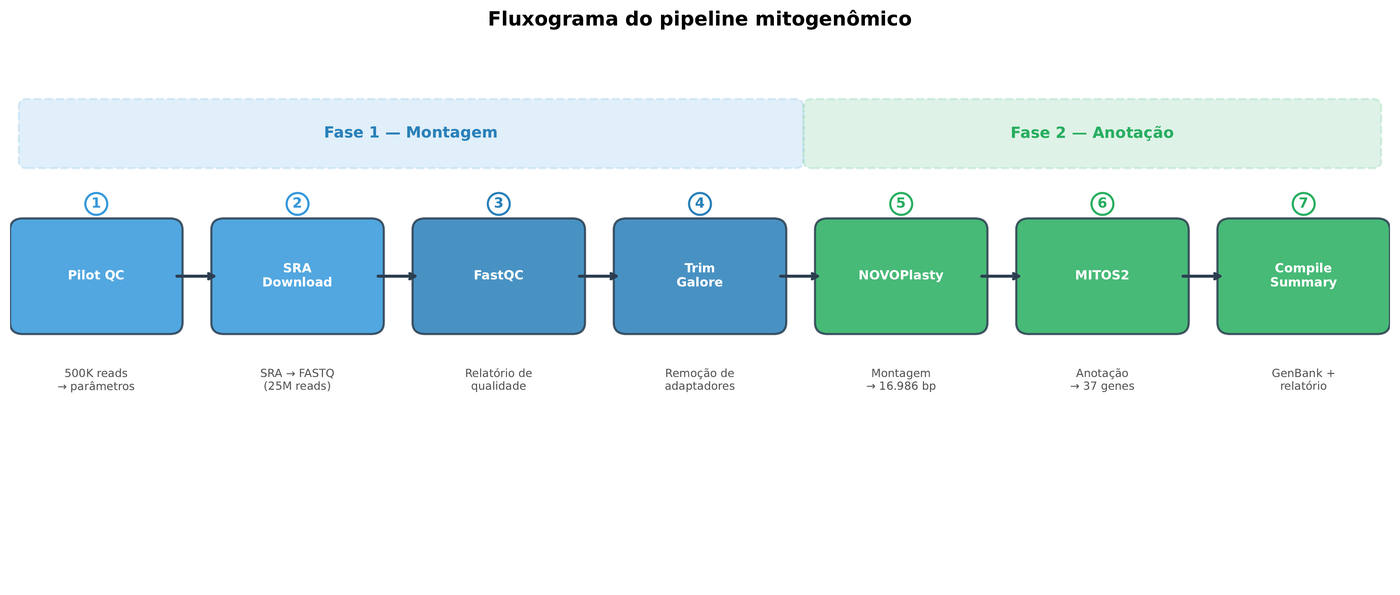
\includegraphics[width=\textwidth]{imagens/fluxograma_pipeline.png}
    \caption{Fluxograma do pipeline com as 7 etapas: Pilot QC, SRA Download, FastQC, Trim Galore, NOVOPlasty, MITOS2 e Compile Summary. Cores distinguem Fase 1 (montagem, azul) e Fase 2 (anotação, verde).}
    \label{fig:fluxograma_pipeline}
\end{figure}

A visão geral do pipeline, representada em formato de fluxograma, ilustra o encadeamento das etapas e destacando a integração entre análise bioinformática e práticas de engenharia de software. Deve-se observar que a lógica condicional do pipeline permite que a etapa de anotação (MITOS2) seja executada apenas quando o banco de dados de referência estiver disponível, tornando a Fase 1 (montagem) independente da Fase 2 (anotação). Adicionalmente, o workflow aplica um \textbf{filtro de circularização}: apenas montagens cujo nome de arquivo inicia com \texttt{Circularized\_assembly} são encaminhadas ao MITOS2 e à compilação de entregáveis. Quando o NOVOPlasty não obtém circularização (produzindo apenas contigs parciais), a anotação é automaticamente omitida, evitando análises sobre montagens incompletas que poderiam gerar resultados biologicamente incorretos. Essa decisão de design garante que os entregáveis finais representem exclusivamente genomas mitocondriais completos e circulares.

\section{Fluxo de Execução do Pipeline}

Esta seção descreve o fluxo completo de execução do pipeline, desde os pré-requisitos até a obtenção dos resultados finais, detalhando as decisões automáticas tomadas pelo sistema e o caminho percorrido pelos dados em cada~etapa.

\subsection{Pré-requisitos e Preparação do Ambiente}

Antes da primeira execução, três preparações são necessárias:

\begin{enumerate}
    \item \textbf{Construção das imagens Docker} --- o repositório inclui cinco Dockerfiles (SRA-Toolkit, FastQC, Trim Galore, NOVOPlasty e MITOS2), cada um com versões pinadas de todas as dependências. A construção é realizada por um script automatizado (\texttt{build\_images.ps1} / equivalente Bash), que gera as imagens localmente sem necessidade de registro externo;
    \item \textbf{Download do banco de dados MITOS2} --- o banco RefSeq89m ($\sim$20~MB compactado) é obtido do Zenodo e extraído em \texttt{data/databases/}. Esse passo é necessário apenas uma vez, pois o banco é reutilizado entre execuções;
    \item \textbf{Configuração do perfil da espécie} --- cada espécie requer um arquivo de configuração em \texttt{conf/} definindo o acesso SRA (\texttt{sra\_accession}), a semente (\texttt{seed}), o intervalo de tamanho esperado (\texttt{genome\_range}), os k-mers a serem tentados (\texttt{novoplasty\_\allowbreak kmers}), o código genético (\texttt{genetic\_code}) e o nome científico (\texttt{organism}).
\end{enumerate}

\subsection{Comando de Execução e Resiliência}

A execução é iniciada por um único comando:

\begin{lstlisting}
nextflow run main.nf -profile <especie>
\end{lstlisting}

Onde \texttt{<espécie>} corresponde ao nome do perfil definido em \texttt{nextflow.config} (e.g., \texttt{a\_leari}, \texttt{test}). Para execuções de longa duração --- típicas em bioinformática, onde o download de dados do SRA pode levar dezenas de minutos e a conversão dos FASTQs pode exceder uma hora ---, o pipeline inclui um script wrapper (\texttt{run\_pipeline.sh}) que encapsula a execução com \texttt{nohup}, permitindo que o terminal seja fechado ou a conexão SSH seja interrompida sem afetar o pipeline. Os logs são automaticamente direcionados para \texttt{logs/<perfil>\_<timestamp>.log}, possibilitando acompanhamento assíncrono via \texttt{tail~-f}.

Para retomar uma execução interrompida, o Nextflow oferece o mecanismo \texttt{-resume}, que reutiliza os resultados de etapas já concluídas armazenados no diretório \texttt{work/}. O pipeline organiza esse diretório por espécie e timestamp (\texttt{work/<espécie>/\allowbreak<timestamp>/}), permitindo identificar e gerenciar execuções individuais. Para retomar uma execução específica, basta indicar o diretório correspondente:

\begin{lstlisting}
nextflow run main.nf -profile <especie> -resume -w work/<especie>/<timestamp>
\end{lstlisting}

\subsection{Fluxo de Dados e Decisões Automáticas}

\begin{figure}[H]
    \centering
    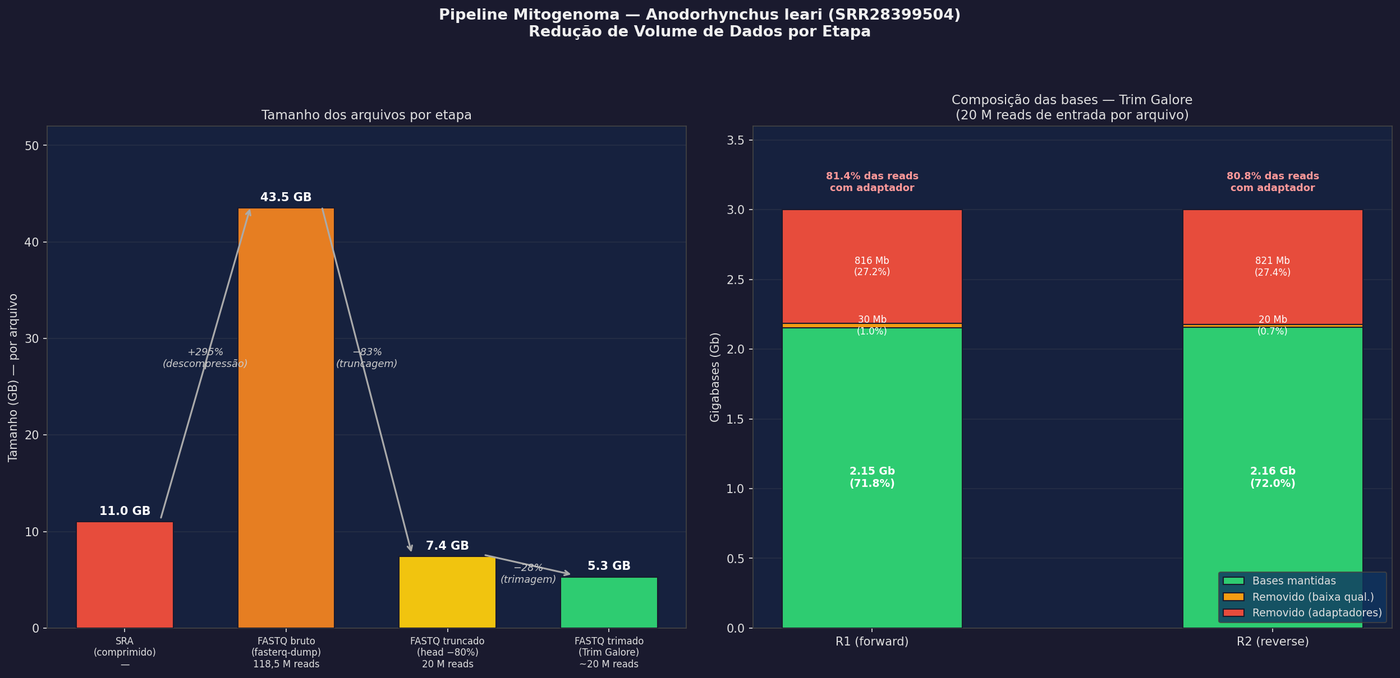
\includegraphics[width=\textwidth]{imagens/reducao_dados_pipeline.png}
    \caption{Fluxo sequencial de dados no pipeline, mostrando os formatos e volumes em cada transição, desde o arquivo \texttt{.sra} (11~GB) até os 14 entregáveis finais (1,6~MB). Destacam-se a redução de 87~GB para 17~KB e os dois pontos de decisão automática.}
    \label{fig:fluxo_dados}
\end{figure}

O pipeline incorpora dois pontos de decisão automática que não requerem intervenção do usuário:

\textbf{Decisão 1 --- Pilot QC (volume de dados).} Quando o parâmetro \texttt{sra\_max\_\allowbreak reads} não é definido no perfil da espécie, o pipeline ativa automaticamente o módulo Pilot QC (seção~\ref{sec:pilotqc}), que baixa uma subamostra de 500.000 leituras, analisa sua qualidade e calcula o número ideal de leituras para a execução principal. Quando o parâmetro é explicitamente definido (e.g., via \texttt{-{}-sra\_max\_\allowbreak reads\allowbreak{} 20000000}), o Pilot QC é pulado e o valor fornecido é utilizado diretamente. Essa lógica condicional é implementada no workflow principal (\texttt{main.nf}) por meio de operadores Nextflow de branching.

\textbf{Decisão 2 --- Filtro de Circularização (qualidade da montagem).} Após a montagem pelo NOVOPlasty, apenas arquivos cujo nome corresponde ao padrão \texttt{Circularized\_\allowbreak assembly\_*} são encaminhados ao MITOS2. Montagens parciais (contigs não circularizados) são automaticamente descartados do fluxo de anotação, evitando que genomas incompletos recebam anotações potencialmente incorretas (e.g., genes truncados nas extremidades de contigs lineares). O pipeline reporta essas montagens parciais no log para que o pesquisador possa investigar manualmente a causa da não-circularização (cobertura insuficiente, semente inadequada, ou regiões repetitivas complexas).

\begin{figure}[H]
    \centering
    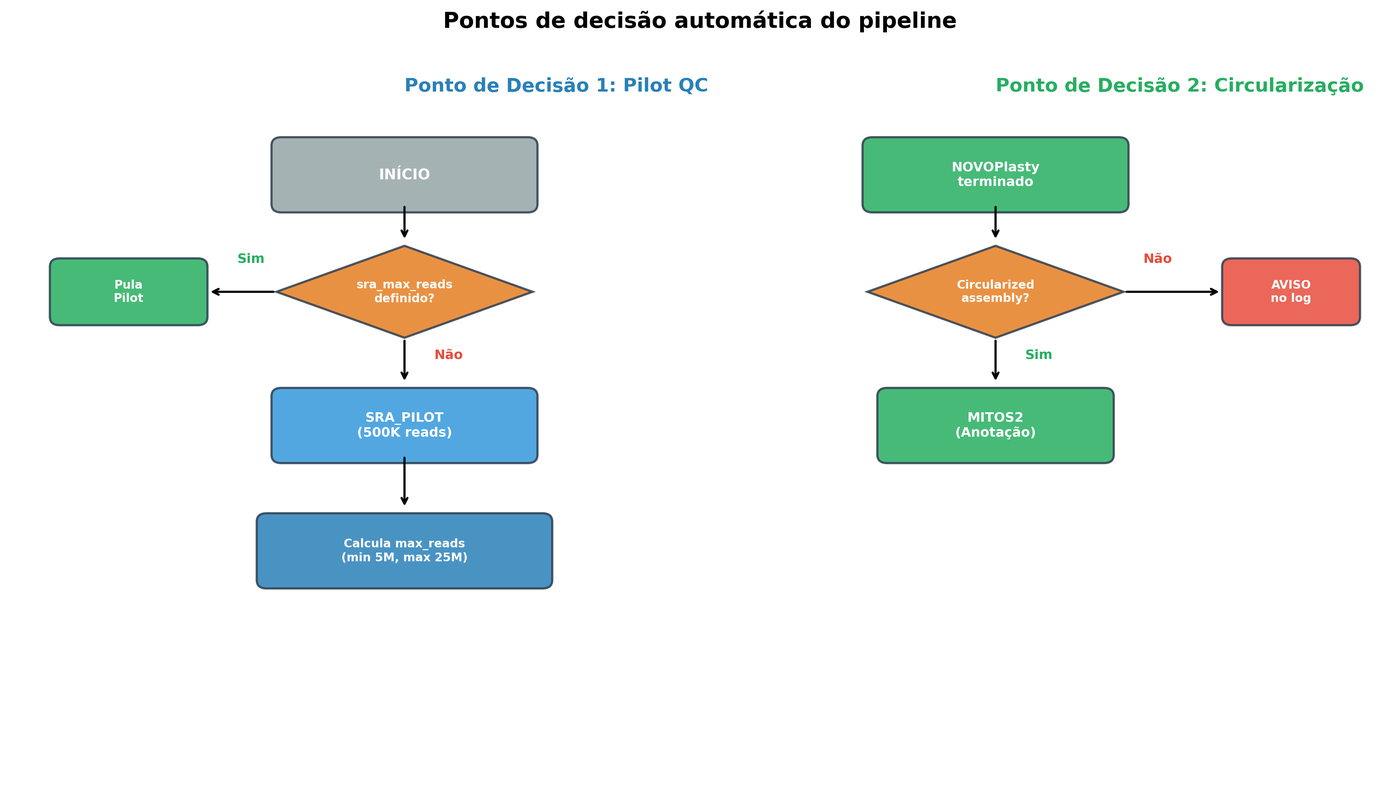
\includegraphics[width=0.85\textwidth]{imagens/diagrama_decisao.png}
    \caption{Diagrama de atividade mostrando os dois pontos de decisão automática do pipeline: (1) Pilot QC --- determina o volume de dados; (2) Filtro de Circularização --- condiciona a anotação à obtenção de genoma circularizado.}
    \label{fig:diagrama_decisao}
\end{figure}

\subsection{Extensibilidade para Novas Espécies}

A adição de uma nova espécie ao pipeline requer apenas a criação de um arquivo de configuração e a obtenção da semente correspondente, sem modificação de código-fonte. Os passos são:

\begin{enumerate}
    \item Identificar no NCBI SRA um dataset de sequenciamento de genoma total para a espécie-alvo;
    \item Localizar o mitogenoma de uma espécie \textbf{congênere} --- isto é, pertencente ao mesmo gênero taxonômico --- (ou filogeneticamente próxima) no NCBI e extrair o gene cox1 como semente;
    \item Criar um arquivo \texttt{conf/<especie>.config} definindo os parâmetros específicos (acesso SRA, semente, genome\_range, k-mers, código genético e nome);
    \item Registrar o novo perfil em \texttt{nextflow.config};
    \item Executar: \texttt{nextflow run main.nf -profile <especie>}.
\end{enumerate}

Essa arquitetura extensível é demonstrada pelas sete sementes incluídas no repositório (\texttt{data/seeds/}), que cobrem espécies de aves, peixes, insetos e nematóides, atestando a generalidade do pipeline para diferentes grupos taxonômicos.

\section{Arquitetura Modular e Scripts do Pipeline}

A organização do código segue a convenção de projetos Nextflow DSL2, em que cada etapa do pipeline corresponde a um \textbf{módulo} independente (arquivo \texttt{.nf} no diretório \texttt{modules/}), e os scripts auxiliares residem no diretório \texttt{scripts/}. Essa separação permite que cada componente seja desenvolvido, testado e mantido de forma isolada. A Tabela~\ref{tab:modulos} apresenta a relação completa dos módulos, scripts e suas responsabilidades.

\begin{longtable}{@{}p{4.5cm}p{2cm}p{7.5cm}@{}}
\caption{Arquitetura modular do pipeline: módulos, scripts e suas responsabilidades.}
\label{tab:modulos} \\
\toprule
\textbf{Arquivo} & \textbf{Tipo} & \textbf{Função} \\
\midrule
\endfirsthead
\caption[]{Arquitetura modular do pipeline (continuação).} \\
\toprule
\textbf{Arquivo} & \textbf{Tipo} & \textbf{Função} \\
\midrule
\endhead
\bottomrule
\endfoot
\texttt{main.nf} & Workflow & Orquestração geral: define a ordem de execução, lógica condicional (Pilot QC, MITOS2) e passagem de dados entre módulos \\
\addlinespace
\texttt{modules/\allowbreak sra\_download.nf} & Módulo & Download do SRA via \texttt{prefetch} + \texttt{fasterq-dump}, com truncamento por \texttt{head} \\
\addlinespace
\texttt{modules/\allowbreak fastqc.nf} & Módulo & Controle de qualidade das leituras brutas via FastQC \\
\addlinespace
\texttt{modules/\allowbreak trim\_galore.nf} & Módulo & Remoção de adaptadores e trimming de qualidade via Trim Galore \\
\addlinespace
\texttt{modules/\allowbreak novoplasty.nf} & Módulo & Montagem iterativa com múltiplos k-mers e re-seeding automático \\
\addlinespace
\texttt{modules/mitos2.nf} & Módulo & Anotação funcional via MITOS2 + geração de SVGs com RNAplot \\
\addlinespace
\texttt{scripts/pilot\_qc.sh} & Script Bash & Análise piloto: calcula Q30\%, taxa de adaptador, fração mitocondrial e recomenda \texttt{max\_reads} \\
\addlinespace
\texttt{scripts/\allowbreak compile\_summary.py} & Script Python & Compila 14 categorias de entregáveis a partir das saídas dos módulos \\
\addlinespace
\texttt{scripts/\allowbreak gff2genbank.py} & Script Python & Converte GFF3 $\rightarrow$ feature table (\texttt{.tbl}) + FASTA formatado (\texttt{.fsa}) para GenBank, com tratamento do frameshift ND3 \\
\addlinespace
\texttt{scripts/\allowbreak generate\_genbank.py} & Script Python & Gera GenBank Flat File (\texttt{.gbk}) e mapa circular (SVG/PDF) via Biopython \\
\addlinespace
\texttt{nextflow.config} & Config. & Parâmetros globais, perfis por espécie, configuração de containers Docker \\
\addlinespace
\texttt{conf/*.config} & Config. & Perfis específicos por espécie (acesso SRA, semente, k-mers, banco MITOS2) \\
\end{longtable}

Essa arquitetura modular permite que novos módulos sejam adicionados (e.g., análise filogenética, BLAST) sem alterar os existentes --- basta criar o arquivo \texttt{.nf}, o Dockerfile correspondente e registrar a chamada no \texttt{main.nf}.

\section{Ferramentas e Tecnologias Utilizadas}

A implementação de um pipeline bioinformático demanda não apenas a escolha de algoritmos adequados, mas também a definição criteriosa de ferramentas que sejam estáveis, bem documentadas e amplamente utilizadas pela comunidade científica. Nesse contexto, a seleção de softwares para este trabalho foi orientada por três princípios fundamentais: (i) funcionalidade biológica, garantindo que cada ferramenta seja apropriada para a etapa que executa, desde a aquisição dos dados até a anotação final do genoma; (ii) confiabilidade e validação prévia, privilegiando programas consolidados na literatura e em uso corrente em pesquisas genômicas; e (iii) compatibilidade com práticas modernas de engenharia de software, assegurando que cada aplicação possa ser encapsulada em containers e integrada a sistemas de gerenciamento de workflows.

Um aspecto central da engenharia deste pipeline é o \textbf{pinamento de versões}. Todas as ferramentas foram encapsuladas em containers Docker com versões explicitamente fixadas, tanto para as imagens base quanto para os softwares instalados. Essa decisão, embora impeça o uso automático de atualizações, garante que o pipeline produza resultados idênticos independentemente do momento ou do ambiente em que for executado, eliminando uma das principais fontes de irreprodutibilidade em bioinformática. A Tabela~\ref{tab:versoes} apresenta as versões de cada componente utilizado.

\begin{table}[H]
\centering
\caption{Versões pinadas dos componentes do pipeline.}
\label{tab:versoes}
\begin{tabular}{@{}lll@{}}
\toprule
\textbf{Componente} & \textbf{Versão} & \textbf{Imagem base} \\
\midrule
SRA-Toolkit & 3.0.10 & ubuntu:22.04 \\
FastQC & 0.12.1 & ubuntu:22.04 \\
Trim Galore & 0.6.10 & ubuntu:22.04 \\
Cutadapt & 4.6 & (dentro do Trim Galore) \\
NOVOPlasty & 4.3.1 & ubuntu:22.04 \\
MITOS2 & 2.1.9 & continuumio/miniconda3:24.1.2-0 \\
ViennaRNA & (via conda) & (dentro do MITOS2) \\
Nextflow & DSL2 (25.x) & --- \\
\bottomrule
\end{tabular}
\end{table}

Além de atender a esses critérios, as ferramentas escolhidas refletem o estado da arte em bioinformática aplicada ao estudo de organelas, cobrindo desde utilitários básicos, como o SRA-Toolkit para acesso a bancos de dados, até plataformas mais complexas, como o NOVOPlasty para montagem especializada de mitogenomas. Da mesma forma, tecnologias transversais como Docker e Nextflow foram incorporadas não pelo papel biológico que desempenham, mas pela sua relevância em assegurar portabilidade, escalabilidade e reprodutibilidade, elementos indispensáveis para a robustez metodológica do pipeline.

Assim, a seguir neste capítulo é descrito de forma integrada as principais ferramentas e tecnologias que compõem o pipeline de montagem de genomas mitocondriais.

\subsection{SRA-Toolkit}

O SRA-Toolkit é o pacote oficial de utilitários do NCBI para manipulação de dados depositados no Sequence Read Archive (SRA), o principal repositório público de dados de sequenciamento de alto rendimento \cite{leinonen2011}. No pipeline desenvolvido, dois utilitários do SRA-Toolkit são empregados em sequência: o \texttt{prefetch}, que realiza o download eficiente do arquivo \texttt{.sra} compactado, e o \texttt{fasterq-dump}, que converte esse arquivo para o formato FASTQ paired-end, compatível com as etapas subsequentes do pipeline.

Uma decisão de implementação relevante diz respeito à estratégia de truncamento de dados. Em datasets de grande volume --- como o utilizado para a arara-azul-de-lear, com 118,5 milhões de pares de leituras (SRR28399504) ---, o processamento integral seria desnecessário e computacionalmente oneroso, dado que o genoma mitocondrial de aves tem cerca de 17~kb e apenas uma fração diminuta das leituras ($\sim$0,17\%) corresponde ao mtDNA. O pipeline implementa, portanto, uma truncagem pós-conversão utilizando o utilitário \texttt{head}, limitando os arquivos FASTQ ao número de leituras definido pelo parâmetro \texttt{sra\_max\_reads}. Essa abordagem foi adotada porque o \texttt{fasterq-dump} do SRA-Toolkit 3.x não implementa o flag \texttt{-X} para limitação na origem, diferentemente do \texttt{fastq-dump} legado, cuja execução é significativamente mais lenta.

A escolha de processar a conversão completa seguida de truncamento, em vez de utilizar o \texttt{fastq-dump} com \texttt{-X}, é justificada pela diferença de desempenho: o \texttt{fasterq-dump} é multi-threaded e até 10 vezes mais rápido que o \texttt{fastq-dump} em datasets grandes \cite{ncbi2023}. O custo adicional de disco temporário é compensado pela economia de tempo e pela confiabilidade da operação, que é automatizada integralmente pelo workflow.

\subsection{FastQC}

O FastQC é uma das ferramentas mais utilizadas na etapa de controle de qualidade de dados de sequenciamento de nova geração (NGS). Desenvolvido pelo Babraham Institute, tornou-se referência para avaliação inicial de leituras em formato FASTQ, sendo amplamente empregado em pipelines de bioinformática devido à sua rapidez, robustez e facilidade de interpretação \cite{andrews2010}.

Do ponto de vista técnico, o FastQC processa os arquivos de entrada em formato FASTQ e gera como saída relatórios em HTML interativo e arquivos compactados (\texttt{.zip}), contendo gráficos e estatísticas sobre diferentes aspectos das sequências. Entre os módulos mais relevantes estão:

\begin{itemize}
    \item \textit{Per base sequence quality}, que avalia a distribuição da qualidade das bases em cada posição do read;
    \item \textit{Per sequence quality scores}, que identifica leituras com baixa qualidade geral;
    \item \textit{Per base GC content}, que compara a distribuição de GC observada com a esperada;
    \item \textit{Overrepresented sequences}, que detecta possíveis contaminantes ou adaptadores;
    \item \textit{Sequence duplication levels}, que informa o grau de redundância entre leituras;
    \item \textit{Adapter content}, que indica a presença de adaptadores de sequenciamento não removidos.
\end{itemize}

Entre as principais vantagens do FastQC estão: (i) a rapidez de execução mesmo em grandes conjuntos de dados, (ii) a geração de relatórios de fácil interpretação, e (iii) a capacidade de identificar múltiplos problemas em uma única execução. No entanto, o programa possui limitações: por ser uma análise pré-alinhamento, não oferece informações sobre a qualidade do mapeamento ou sobre a distribuição de leituras no genoma de referência. Além disso, os resultados devem ser interpretados com cautela, já que pequenas variações em métricas, como o conteúdo GC, podem refletir características biológicas legítimas e não necessariamente artefatos técnicos.

A escolha pelo FastQC neste trabalho se justifica por sua ampla aceitação na comunidade científica como ferramenta de triagem inicial de qualidade. Sua aplicação permite identificar rapidamente problemas técnicos, orientar a necessidade de trimming ou filtragem, e garantir que apenas leituras de qualidade adequada sejam utilizadas nas etapas de montagem do mitogenoma. Dessa forma, o FastQC atua como um ponto de controle essencial para assegurar a confiabilidade das análises subsequentes.

\subsection{Cutadapt e Trim Galore}

Após a avaliação inicial da qualidade das leituras, pode ser necessário realizar etapas de filtragem para remover \textbf{adaptadores} residuais e \textbf{bases de baixa qualidade}. Para compreender essas operações, é necessário esclarecer dois conceitos fundamentais.

\textbf{Adaptadores} são sequências sintéticas curtas (tipicamente 30--60 nucleótidos) que são quimicamente ligadas às extremidades dos fragmentos de DNA durante a preparação da biblioteca de sequenciamento. Funcionam como ``ancoradouros'' que permitem ao sequenciador reconhecer e processar cada fragmento. Após o sequenciamento, essas sequências artificiais não fazem parte do genoma do organismo e precisam ser removidas antes da montagem, pois sua presença geraria sobreposições falsas entre leituras, comprometendo a reconstrução do genoma.

\textbf{Bases de baixa qualidade} referem-se a nucleótidos cuja identificação pelo sequenciador apresenta baixa confiança. A qualidade de cada base é expressa pela \textbf{pontuação Phred} ($Q$), uma escala logarítmica em que:

\begin{equation}
Q = -10 \log_{10}(P)
\label{eq:phred}
\end{equation}

\noindent sendo $P$ a probabilidade de erro \cite{ewing1998}. Assim, $Q = 20$ indica 1\% de probabilidade de erro (99\% de acerto), enquanto $Q = 30$ indica 0,1\% de erro (99,9\% de acerto). Bases com $Q < 20$ são geralmente consideradas de baixa qualidade e removidas no processo de \textbf{trimming} (corte) --- a operação de remoção sistemática de adaptadores e bases de baixa qualidade das extremidades das leituras.

Nesse contexto, duas ferramentas complementares são utilizadas no pipeline: Cutadapt e Trim Galore.

O Cutadapt é um programa desenvolvido por \citeonline{martin2011} especificamente para identificar e remover sequências de adaptadores em dados de alto rendimento. As leituras geradas por tecnologias como Illumina frequentemente contêm fragmentos de adaptadores ligados durante a preparação da biblioteca, que, se não forem removidos, podem comprometer a montagem ou o mapeamento subsequente. O Cutadapt utiliza algoritmos de busca eficiente para detectar esses fragmentos nas extremidades das leituras e removê-los, além de permitir o corte de bases de baixa qualidade de acordo com pontuações Phred. Como entrada, o programa recebe arquivos \textbf{FASTQ} --- formato de texto que armazena tanto a sequência de cada leitura quanto a qualidade Phred de cada base individual, representada por caracteres ASCII ---, e como saída gera novos FASTQ já filtrados, prontos para análises subsequentes.

O Trim Galore é um wrapper que automatiza a execução do Cutadapt em conjunto com o FastQC, simplificando o processo de trimming e tornando-o mais acessível ao usuário \cite{babraham2019}. Com ele, é possível remover adaptadores mesmo quando a sequência exata não é previamente conhecida, o que é particularmente útil em experimentos com bibliotecas de origem diversa. Além disso, o Trim Galore aplica rotinas de filtragem por qualidade e integra relatórios do FastQC para avaliar o impacto do corte.

Entre as principais vantagens do Cutadapt e do Trim Galore estão: (i) a remoção precisa de adaptadores, prevenindo erros de montagem, (ii) a flexibilidade de configuração de parâmetros, e (iii) a integração automatizada que reduz a intervenção manual. Suas limitações incluem a necessidade de escolher cuidadosamente os limiares de qualidade, já que cortes excessivos podem resultar em perda de informação biológica relevante, enquanto cortes insuficientes podem deixar contaminantes residuais.

A escolha por essas ferramentas neste trabalho se justifica pelo seu amplo uso na comunidade científica e pela confiabilidade de seus resultados. A integração de Cutadapt e Trim Galore garante que as leituras que avançam para a montagem apresentem qualidade adequada, reduzindo o risco de artefatos e aumentando a robustez dos resultados obtidos pelo pipeline.

\subsection{NOVOPlasty}

O NOVOPlasty é um montador especializado desenvolvido para reconstrução de genomas de organelas, como mitocôndrias e cloroplastos, a partir de dados de sequenciamento de genoma total. Publicado por \citeonline{dierckxsens2017}, tornou-se uma das ferramentas mais amplamente utilizadas para esse fim devido à sua eficiência e facilidade de uso.

Do ponto de vista técnico, o NOVOPlasty baseia-se na estratégia seed-and-extend. O processo de montagem é iniciado a partir de uma sequência fornecida pelo usuário --- denominada seed --- que pode ser um fragmento do genoma da organela em estudo, uma sequência de uma espécie próxima ou até mesmo uma sequência completa de organela de outro organismo. A partir dessa seed, o software realiza uma extensão bidirecional, identificando leituras sobrepostas e construindo gradualmente a sequência circular completa do genoma. Para acelerar o processo, o programa utiliza tabelas de hash, que permitem buscas rápidas por sobreposições entre as leituras.

O NOVOPlasty recebe como entrada arquivos FASTQ contendo leituras pareadas, bem como um arquivo FASTA com a sequência seed. A saída consiste em um arquivo FASTA representando o genoma circularizado, acompanhado de arquivos de log e, em alguns casos, múltiplas opções de montagem (quando diferentes caminhos são possíveis no grafo de montagem).

Entre as principais vantagens do NOVOPlasty destacam-se: (i) sua alta eficiência na recuperação de genomas completos de organelas mesmo a partir de dados de genoma total, (ii) a baixa exigência de parâmetros complexos, o que o torna acessível a usuários com diferentes níveis de experiência, e (iii) a capacidade de lidar com diferentes tipos de sementes, permitindo flexibilidade em estudos de espécies com genomas pouco conhecidos. No entanto, como limitações, pode-se destacar: (i) a dependência da qualidade e da escolha adequada da seed, que influencia diretamente o sucesso da montagem, e (ii) o risco de circularizações incorretas em casos de regiões altamente repetitivas ou coberturas desbalanceadas.

No pipeline implementado, o módulo NOVOPlasty incorpora uma lógica iterativa com re-seeding automático: caso a primeira execução não resulte em circularização, o maior contig obtido é automaticamente utilizado como nova semente em uma segunda tentativa, e múltiplos valores de k-mer são experimentados em sequência. Essa estratégia aumenta a taxa de sucesso da montagem sem requerer intervenção manual do usuário.

\subsection{MITOS2}

O MITOS2 é uma ferramenta desenvolvida para a anotação funcional de genomas mitocondriais em metazoários. Apresentada por \citeonline{donath2019}, constitui a evolução da primeira versão do MITOS, oferecendo maior precisão na predição de genes, integração com bases de dados atualizadas e maior flexibilidade de execução.

Tecnicamente, o MITOS2 combina métodos de homologia (comparação com sequências conhecidas) e algoritmos de predição \textit{ab initio} (a partir da própria sequência, sem referência externa) para identificar as principais classes de genes presentes em genomas mitocondriais. O sistema utiliza alinhamentos com modelos de substituição específicos para proteínas codificadas por mitocôndrias, além de perfis de RNA para identificar rRNAs e tRNAs por meio de modelos de covariância (Infernal). As entradas consistem em um arquivo FASTA contendo a sequência do genoma mitocondrial a ser anotado, e as saídas incluem: (i) arquivos tabulares com as coordenadas dos genes anotados, (ii) representações gráficas do genoma mostrando a organização gênica, e (iii) arquivos de anotação em formatos padrão, como GFF3 e BED (formato tabular simplificado com coordenadas genômicas). É relevante notar que, conforme demonstrado por \citeonline{donath2019}, as anotações do RefSeq contêm erros --- em particular, atribuições implausíveis de posições de códons de início e parada, além de uma fração substancial de anotações incompletas que identificam apenas fragmentos de genes codificadores de proteínas. O MITOS2 demonstrou que uma anotação totalmente automática com acurácia muito alta é possível, representando uma melhoria drástica em relação à determinação manual de fronteiras gênicas.

A versão empregada neste trabalho (v2.1.9) foi instalada via Conda em um container Docker baseado em Miniconda 24.1.2-0, utilizando o banco de dados RefSeq89m obtido do Zenodo \cite{donath2019}. Essa abordagem garante que a ferramenta, normalmente executada via interface web, funcione de forma autônoma em linha de comando e completamente integrada ao workflow Nextflow.

Como extensão funcional, o pipeline integra automaticamente a geração de representações visuais da estrutura secundária dos tRNAs e rRNAs preditos. Para isso, o módulo MITOS2 extrai as sequências e estruturas dot-bracket dos arquivos de saída e as processa com o RNAplot, componente do pacote ViennaRNA \cite{lorenz2011}, gerando arquivos SVG individuais para cada RNA não codificante. Essa funcionalidade, originalmente disponível apenas na versão web do MITOS2 (UseGalaxy), foi reproduzida localmente no pipeline, garantindo que os diagramas de estrutura secundária sejam gerados sem dependência de serviços externos.

Entre as principais vantagens do MITOS2 destacam-se: (i) a automação completa da etapa de anotação, reduzindo a necessidade de curadoria manual extensiva; (ii) a compatibilidade com diferentes grupos taxonômicos de metazoários; e (iii) a produção de relatórios gráficos de fácil interpretação. Em estudos recentes de genômica mitocondrial comparativa, a anotação do MITOS2 é frequentemente complementada pela verificação de tRNAs com tRNAscan-SE, ferramenta especializada que utiliza modelos de covariância otimizados para a predição de RNAs transportadores \cite{zhan2024,kundu2024,shi2024}. Essa combinação MITOS2 + tRNAscan-SE tem se consolidado como padrão metodológico na área. No presente pipeline, o MITOS2 é utilizado como ferramenta única de anotação, dado que seus próprios modelos de covariância (via Infernal) já incorporam predição de tRNAs com alta sensibilidade; a integração opcional de tRNAscan-SE como módulo de verificação adicional constitui uma perspectiva futura. Por outro lado, como limitações, pode apresentar divergências em regiões com estruturas gênicas incomuns --- como o caso do gene ND3 em aves, que apresenta um \textbf{frameshift insertion} (inserção de um nucleotídeo que desloca o quadro de leitura do código genético, alterando a sequência de aminoácidos traduzida daquele ponto em diante), documentado por \citeonline{mindell1998}, levando o MITOS2 a reportar o gene como dois \textbf{ORFs} (\textit{Open Reading Frames} --- quadros abertos de leitura, trechos de DNA que potencialmente codificam proteínas) distintos (nad3\_0 e nad3\_1) em vez de um único CDS (\textit{Coding Sequence} --- sequência codificante) com \texttt{join()}. Esse tipo de situação requer validação complementar e tratamento específico na conversão para formatos de submissão ao GenBank.

\subsection{Docker}

No pipeline proposto, cada ferramenta foi encapsulada em um container Docker, assegurando que todas as dependências fossem executadas em ambientes controlados e consistentes \cite{merkel2014}. O pipeline utiliza cinco imagens Docker distintas, cada uma correspondendo a um estágio do processamento, conforme apresentado na Tabela~\ref{tab:docker}.

\begin{table}[H]
\centering
\caption{Imagens Docker utilizadas no pipeline.}
\label{tab:docker}
\footnotesize
\resizebox{\textwidth}{!}{%
\begin{tabular}{@{}llll@{}}
\toprule
\textbf{Imagem} & \textbf{Base} & \textbf{Ferramenta} & \textbf{Dockerfile} \\
\midrule
\texttt{mitogenome-pipeline/sra-tools:1.0} & ubuntu:22.04 & SRA-Toolkit 3.0.10 & \texttt{docker/sra-tools/} \\
\addlinespace
\texttt{mitogenome-pipeline/fastqc:1.0} & ubuntu:22.04 & FastQC 0.12.1 & \texttt{docker/fastqc/} \\
\addlinespace
\texttt{mitogenome-pipeline/trim-galore:1.0} & ubuntu:22.04 & Trim Galore 0.6.10 + Cutadapt 4.6 & \texttt{docker/trim-galore/} \\
\addlinespace
\texttt{mitogenome-pipeline/novoplasty:1.0} & ubuntu:22.04 & NOVOPlasty 4.3.1 & \texttt{docker/novoplasty/} \\
\addlinespace
\texttt{mitogenome-pipeline/mitos2:1.0} & miniconda3:24.1.2-0 & MITOS2 2.1.9 + ViennaRNA & \texttt{docker/mitos2/} \\
\bottomrule
\end{tabular}}%
\end{table}

Essa abordagem eliminou a necessidade de configurações manuais complexas e garantiu que softwares como FastQC, Cutadapt, NOVOPlasty e MITOS2 operassem de forma uniforme em diferentes sistemas operacionais. Com isso, a montagem e a anotação de mitogenomas tornam-se replicáveis em qualquer ambiente computacional que disponha do Docker instalado, ampliando a portabilidade do pipeline.

\subsection{Nextflow}

A orquestração do pipeline foi implementada no Nextflow DSL2, que estruturou os processos em módulos independentes (um arquivo \texttt{.nf} por etapa), conectando automaticamente suas entradas e saídas \cite{ditommaso2017}. Essa organização permitiu automatizar a lógica iterativa da montagem, como a possibilidade de reaproveitar contigs parciais do NOVOPlasty como novas seeds em execuções subsequentes. Além disso, o Nextflow possibilitou a paralelização de tarefas, a retomada de execuções interrompidas (via flag \texttt{-resume}) e a integração direta com containers Docker. Dessa forma, o pipeline desenvolvido combina simplicidade de uso com escalabilidade e reprodutibilidade, adequando-se tanto a computadores locais quanto a servidores de alto desempenho.

O sistema de perfis do Nextflow foi utilizado para parametrizar execuções distintas sem alterar o código-fonte. Cada espécie estudada possui um arquivo de configuração próprio (e.g., \texttt{conf/a\_leari.config}) contendo os parâmetros específicos --- acesso SRA, semente, tamanho esperado do genoma, código genético --- que são carregados automaticamente ao invocar o perfil correspondente (\texttt{nextflow run main.nf -profile a\_leari}).

\subsection{GitHub}

O GitHub é uma plataforma de hospedagem de código baseada no sistema de controle de versão Git, amplamente utilizada para o desenvolvimento colaborativo de software e projetos científicos. Para pipelines de bioinformática, a disponibilização em um repositório GitHub garante não apenas transparência, mas também acessibilidade e manutenção a longo prazo.

Neste trabalho, o GitHub foi utilizado como repositório público para disponibilizar o pipeline desenvolvido, assegurando sua acessibilidade, versionamento e documentação adequada. Essa prática se alinha às diretrizes de ciência aberta e reforça o compromisso com a reprodutibilidade e a transparência metodológica. O repositório inclui: o código completo do workflow Nextflow, todos os Dockerfiles, scripts auxiliares, configurações de perfil por espécie, dados de semente (sequências cox1), documentação e guia de execução.

Adicionalmente, o sistema de branches do Git foi utilizado para preservar estados estáveis do pipeline: a branch \texttt{fase1-montagem} contém o estado validado da Fase 1 (apenas montagem, sem anotação), enquanto a branch \texttt{main} contém o pipeline completo com todas as etapas integradas.

\section{Aquisição e Preparo dos Dados}

A primeira etapa prática do pipeline consiste na aquisição e organização dos dados de sequenciamento que servirão de insumo para a montagem dos genomas mitocondriais. Para este trabalho, foram utilizados datasets públicos provenientes do Sequence Read Archive (SRA), repositório mantido pelo NCBI e reconhecido como um dos principais bancos internacionais de dados de sequenciamento de alto rendimento \cite{leinonen2011}. A escolha por dados públicos justifica-se pela sua ampla disponibilidade, pela diversidade de organismos representados e pela possibilidade de reproduzir e validar resultados obtidos em trabalhos prévios.

O acesso aos dados é realizado por meio do SRA-Toolkit v3.0.10 (encapsulado em container Docker), por meio de dois comandos sequenciais: \texttt{prefetch}, responsável pelo download do arquivo \texttt{.sra} compactado, e \texttt{fasterq-dump}, que converte o arquivo para o formato FASTQ paired-end. Implementou-se também a estratégia de retries automáticos (até 2 tentativas) para lidar com instabilidades de rede, comuns em downloads de datasets grandes do NCBI.

Como estudo de caso principal, foi utilizado o dataset SRR28399504 referente ao genoma da arara-azul-de-lear (\textit{Anodorhynchus leari}), gerado por sequenciamento paired-end na plataforma Illumina HiSeq X Ten \cite{iridian2024}, com leituras de 150 pares de bases e um total de 118,5 milhões de pares. Para validação do pipeline, foi utilizado o dataset SRR36182901 referente a \textit{Diploprion bifasciatus} (peixe-sabão barrado), gerado em plataforma NovaSeq X Plus com leituras de 151~bp.

\section{Análise Piloto de Qualidade (Pilot QC)}
\label{sec:pilotqc}

Uma inovação incorporada ao pipeline é o módulo de análise piloto de qualidade, que soluciona um problema prático recorrente em montagens de organelas: a determinação do volume adequado de dados a serem processados. Em datasets de sequenciamento de genoma total, a proporção de leituras mitocondriais é tipicamente inferior a 1\% \cite{dierckxsens2017}, o que significa que processar integralmente um dataset de 100~GB resultaria em centenas de gigabytes de dados nucleares irrelevantes para a montagem do mitogenoma. Além da ineficiência computacional, esse volume torna a análise impraticável em computadores pessoais: um notebook com 256~GB de SSD e 16~GB de RAM não comportaria os arquivos temporários gerados pela conversão e processamento de 87~GB de FASTQs brutos. O Pilot QC resolve esse problema logo na primeira etapa, reduzindo drasticamente o volume de dados antes que qualquer processamento pesado ocorra.

O módulo Pilot QC opera da seguinte forma: quando o parâmetro \texttt{sra\_max\_reads} não é definido pelo usuário, o pipeline baixa automaticamente uma subamostra de 500.000 leituras (aproximadamente 500~MB) utilizando o \texttt{fastq-dump -X}, que limita o download na origem sem necessidade de transferir o dataset completo. A escolha do \texttt{fastq-dump} (em vez do \texttt{fasterq-dump} utilizado no módulo de download principal) é deliberada: o \texttt{fastq-dump}, embora mais lento, suporta o flag \texttt{-X} que restringe o download na origem, evitando transferir o dataset completo. Já o \texttt{fasterq-dump}, utilizado no download principal por ser multi-threaded e até 10 vezes mais rápido \cite{ncbi2023}, não implementa esse flag, exigindo a estratégia de truncamento pós-conversão via \texttt{head}. Para amostras piloto de 500~K reads, a menor velocidade do \texttt{fastq-dump} é irrelevante (execução em segundos), tornando a escolha ótima para cada contexto. Essa subamostra é então submetida ao script \texttt{scripts/pilot\_qc.sh}, um analisador desenvolvido inteiramente em Bash que opera diretamente sobre os arquivos FASTQ sem dependências externas além de \texttt{awk} e \texttt{grep}. O script extrai três métricas-chave:

\begin{enumerate}
    \item \textbf{Proporção de bases com qualidade $\geq$ Q30}, indicando a qualidade geral das leituras;
    \item \textbf{Proporção de leituras com adaptador Illumina TruSeq} residual, estimando a perda efetiva no trimming;
    \item \textbf{Fração mitocondrial estimada}, calculada por correspondência de k-mers da sequência semente contra as leituras piloto.
\end{enumerate}

A partir dessas métricas, o script calcula o número total de leituras necessário para atingir uma cobertura-alvo de 500$\times$ no mitogenoma, aplicando fatores de correção por qualidade e por presença de adaptador, com uma margem de segurança de 1,5$\times$. O resultado é limitado ao intervalo de 5 a 50 milhões de leituras. Esse valor é então passado automaticamente ao módulo de download principal, que trunca os FASTQs no número calculado.

A fórmula para o número de leituras mitocondriais necessárias é:

\begin{equation}
R_{mito} = \frac{C_{alvo} \times G}{L \times 2}
\label{eq:rmito}
\end{equation}

\noindent e o número total de leituras a serem baixadas é:

\begin{equation}
R_{total} = \frac{R_{mito} \times F_{Q30} \times F_{adapter}}{f_{mito}} \times 1{,}5
\label{eq:rtotal}
\end{equation}

\noindent onde $C_{alvo}$ é a cobertura desejada, $G$ é o tamanho médio esperado do genoma, $L$ é o comprimento médio das leituras, $f_{mito}$ é a fração mitocondrial estimada, e $F_{Q30}$ e $F_{adapter}$ são fatores de correção baseados na qualidade e presença de adaptadores.

Caso o usuário opte por definir manualmente o \texttt{sra\_max\_reads} via parâmetro de linha de comando, a etapa Pilot QC é automaticamente pulada, preservando a flexibilidade para cenários em que o pesquisador já possui conhecimento prévio sobre seus dados.

\begin{figure}[H]
    \centering
    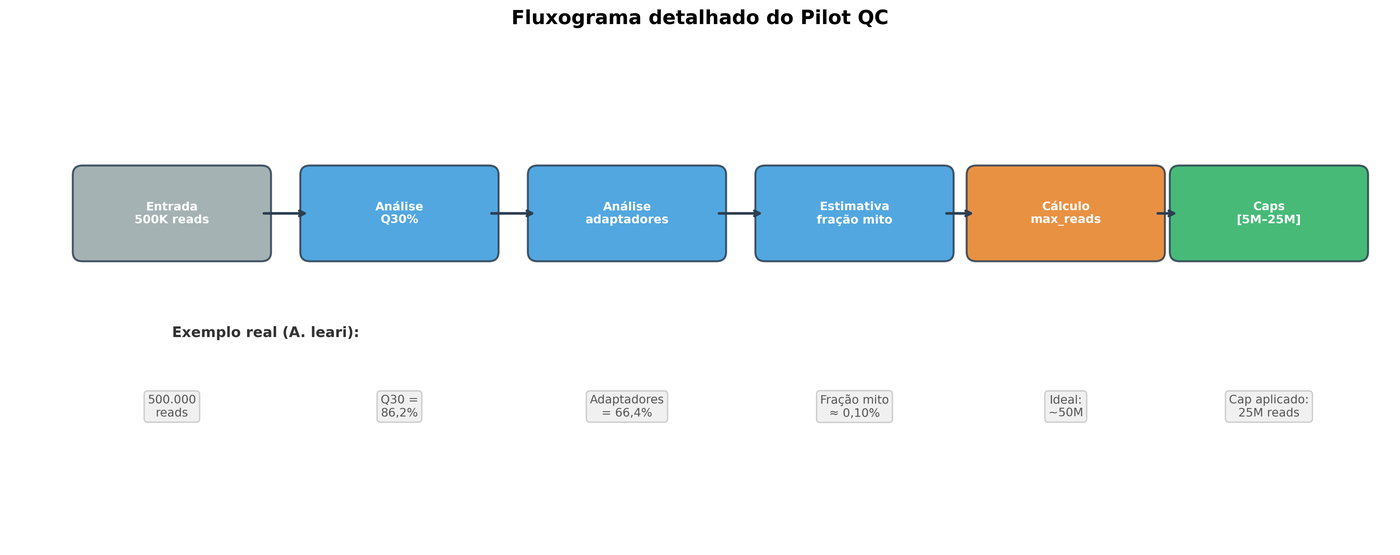
\includegraphics[width=0.85\textwidth]{imagens/pilot_qc_detalhado.png}
    \caption{Fluxograma de decisão do Pilot QC: análise de Q30\%, taxa de adaptadores e fração mitocondrial estimada para cálculo automático do número ideal de leituras, com caps entre 5M e 25M.}
    \label{fig:pilot_qc}
\end{figure}

\section{Controle de Qualidade e Pré-processamento}

Após a aquisição e organização dos dados de sequenciamento, a etapa seguinte do pipeline consiste na avaliação da qualidade das leituras e na aplicação de procedimentos de filtragem. Essa fase é essencial para assegurar que apenas dados confiáveis avancem para a montagem do genoma mitocondrial, evitando que artefatos técnicos comprometam a acurácia do resultado final.

O primeiro passo é a execução do FastQC v0.12.1, que gera relatórios interativos em HTML contendo métricas fundamentais para a avaliação da qualidade das leituras. Em seguida, é aplicado o Trim Galore v0.6.10 (que integra o Cutadapt v4.6), com parâmetros de qualidade Phred mínimo de 20 e comprimento mínimo de leitura de 50~bp para remoção de adaptadores e bases de baixa qualidade. No módulo implementado, o número de threads de CPU foi deliberadamente limitado a 2 para evitar ultrapassar a alocação de CPU no container, dado que o Trim Galore gera internamente threads adicionais para compressão (pigz) e para o próprio Cutadapt.

Além de aumentar a confiabilidade biológica das leituras, o pré-processamento contribui significativamente para a redução do volume de dados. Na execução para a arara-azul-de-lear, por exemplo, o Trim Galore detectou adaptadores Illumina TruSeq em 81,4\% das leituras, e após o trimming, 71,9\% das bases foram mantidas --- uma redução de volume de $\sim$28\%.

\section{Montagem do Mitogenoma}

A montagem do genoma mitocondrial constitui a etapa central do pipeline, pois é nela que se obtém a sequência circular completa que serve de base para a anotação funcional e análises comparativas. Para essa finalidade é utilizado o NOVOPlasty v4.3.1, um dos montadores mais consolidados para organelas \cite{dierckxsens2017}.

No pipeline implementado, o módulo NOVOPlasty incorpora diversas melhorias em relação ao uso padrão da ferramenta:

\begin{enumerate}
    \item \textbf{Múltiplos k-mers}: o parâmetro \texttt{novoplasty\_kmers} permite definir uma lista de valores de k-mer a serem tentados em sequência (e.g., \texttt{'39,33'}). O pipeline experimenta cada um até obter circularização;
    \item \textbf{Re-seeding automático}: para cada k-mer, caso a primeira execução não circularize, o maior contig obtido é automaticamente extraído e utilizado como nova semente em até 5 iterações (configurável);
    \item \textbf{Liberação de espaço}: após a montagem, os arquivos FASTQ trimados são automaticamente deletados para economizar espaço em disco, comportamento crucial para execuções com dados volumosos.
\end{enumerate}

A seleção dos valores de k-mer segue as recomendações do próprio NOVOPlasty \cite{dierckxsens2017}, que aceita valores ímpares no intervalo de 21 a 39. Valores maiores de k-mer (como 39) favorecem a \textbf{especificidade} da montagem --- cada k-mer é mais longo e, portanto, menos ambíguo, reduzindo o risco de quimeras e extensões incorretas. Por outro lado, valores menores (como 33) aumentam a \textbf{sensibilidade}, permitindo extensões em regiões de menor cobertura ou maior divergência entre a semente e o genoma-alvo. Assim, a estratégia adotada neste pipeline inicia pelo valor máximo (39), que produz montagens mais confiáveis quando a cobertura e a qualidade dos dados são adequadas, e recorre ao valor menor (33) apenas se a circularização não for alcançada na primeira tentativa. Para a arara-azul-de-lear, a circularização ocorreu na primeira tentativa com k-mer 39, indicando que a cobertura de 306$\times$ e a qualidade do HiSeq X Ten foram suficientes para o valor mais restritivo. Já para \textit{D.~bifasciatus}, a circularização ocorreu com k-mer 33, possivelmente refletindo diferenças na cobertura ou na composição nucleotídica do dataset.

\begin{figure}[H]
    \centering
    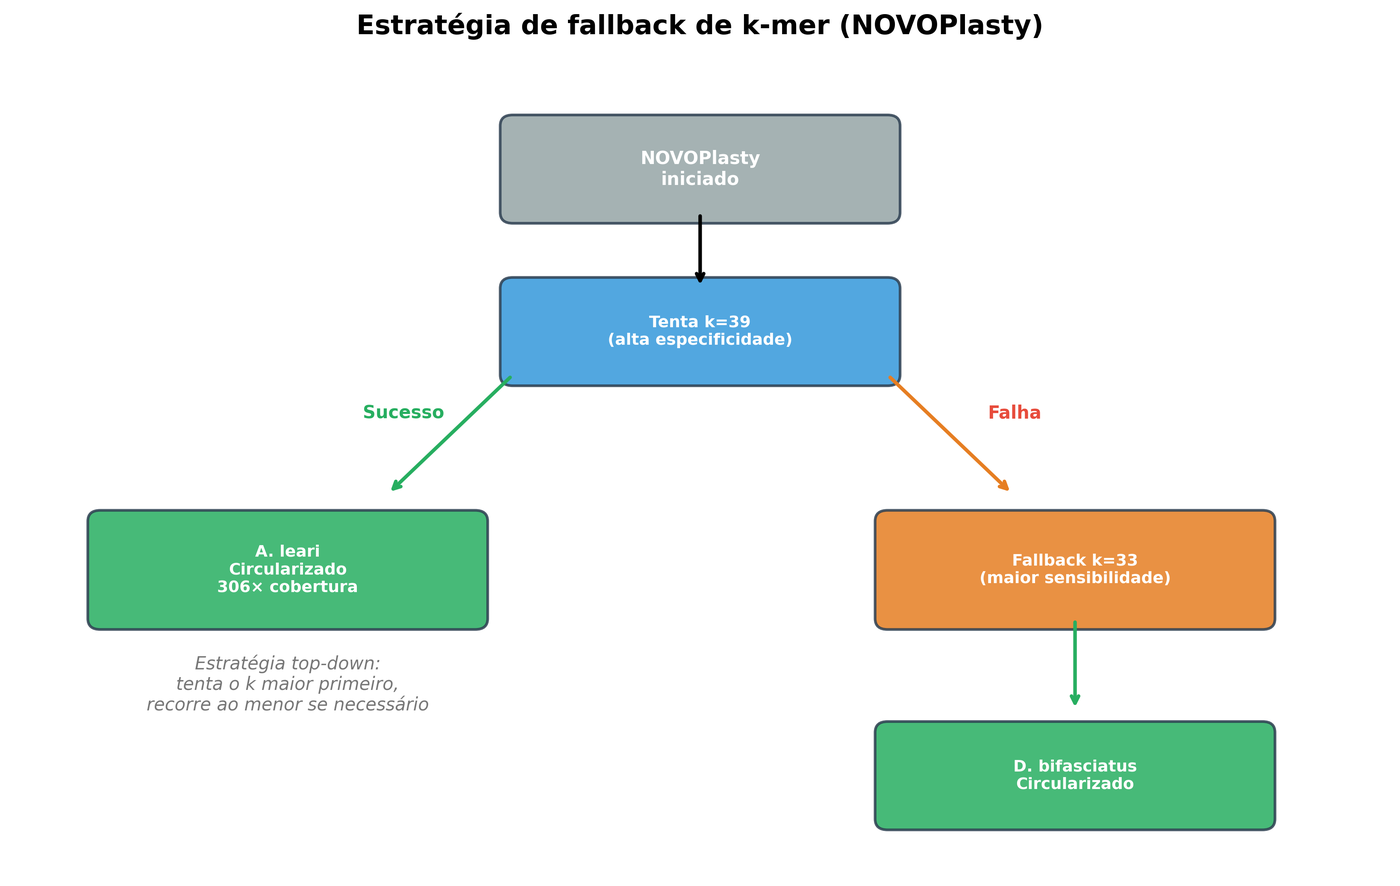
\includegraphics[width=0.85\textwidth]{imagens/kmer_fallback.png}
    \caption{Diagrama da lógica iterativa de k-mers: tentativa com k=39 (alta especificidade) seguida de \textit{fallback} para k=33 (maior sensibilidade) quando a circularização não é alcançada.}
    \label{fig:kmer_fallback}
\end{figure}

\textbf{Obtenção da semente (seed).} O NOVOPlasty requer uma sequência inicial conhecida para ancorar a extensão. A estratégia adotada neste trabalho consiste em: (i) identificar no NCBI uma espécie congênere ou filogeneticamente próxima que possua mitogenoma completo depositado; (ii) extrair o gene cox1 dessa referência, por ser o marcador mitocondrial mais conservado e amplamente disponível; e (iii) salvar a região em formato FASTA. Para a arara-azul-de-lear, foi utilizado o gene cox1 de \textit{A.~hyacinthinus} (NC\_082165.1, posições 5359--6906, 1.548~bp), espécie congênere cuja proximidade filogenética garante homologia suficiente para o seed-and-extend funcionar eficazmente. Para \textit{D.~bifasciatus}, foi utilizado o próprio cox1 da referência publicada (PZ143763.1, 1.560~bp). O repositório do pipeline inclui um guia detalhado para obtenção de sementes (\texttt{data/seeds/COMO\_OBTER\_SEMENTE.md}) e exemplos para sete espécies de diferentes grupos taxonômicos.

\textbf{Seleção do intervalo de tamanho (\texttt{genome\_range}).} O NOVOPlasty utiliza um intervalo esperado de tamanho do genoma para descartar extensões espúrias. A determinação desse intervalo segue a mesma lógica da semente: busca-se no NCBI o tamanho do mitogenoma de referência da espécie congênere mais próxima e aplica-se uma margem de $\pm$1.500--2.000~bp para acomodar variação interespecífica. Para a arara-azul-de-lear, a referência \textit{A.~hyacinthinus} (16.999~bp) resultou no intervalo 15.500--18.500~bp; para \textit{D.~bifasciatus}, a referência PZ143763.1 (16.805~bp) resultou em 15.000--18.500~bp.

\textbf{Parâmetro \texttt{insert\_size}.} O tamanho do inserto da biblioteca é parametrizado como 300~bp (valor padrão conservador para preparações Illumina). O NOVOPlasty utiliza esse valor como estimativa inicial, mas refina-o automaticamente durante a montagem --- no caso da arara-azul-de-lear, o inserto real medido foi de 213~bp, sem impacto na qualidade da circularização.

\section{Anotação Funcional}

Concluída a etapa de montagem, procede-se à anotação funcional do genoma mitocondrial reconstruído, utilizando o MITOS2 v2.1.9 com o banco de dados RefSeq89m. A anotação é executada automaticamente pelo pipeline quando o parâmetro \texttt{mitos2\_db} está configurado, sendo condicional para permitir que a Fase 1 (montagem) opere independentemente.

O módulo MITOS2 recebe como entrada o arquivo FASTA da montagem circularizada e produz como saída: arquivo GFF3 com coordenadas dos genes, tabelas BED, sequências proteicas preditas (FAA), mapa linear do genoma (PNG) e plots de qualidade (PDF). Adicionalmente, o pipeline gera automaticamente diagramas SVG da estrutura secundária prevista para cada tRNA e rRNA identificado, utilizando o programa RNAplot do pacote ViennaRNA.

O código genético é parametrizado (\texttt{genetic\_code = 2} para vertebrados mitocondriais, \texttt{genetic\_code = 5} para invertebrados), permitindo que o mesmo pipeline seja utilizado para diferentes grupos taxonômicos sem modificação de código.

\section{Compilação dos Entregáveis}

Uma funcionalidade diferenciada do pipeline é a compilação automática de todos os produtos da análise em uma pasta organizada de entregáveis (\texttt{summary/}), pronta para apresentação acadêmica ou submissão a bancos de dados. Essa etapa é executada pelo módulo \texttt{COMPILE\_SUMMARY}, que integra três scripts Python:

\begin{enumerate}
    \item \textbf{\texttt{gff2genbank.py}} --- Converte a anotação GFF3 do MITOS2 para o formato feature table (\texttt{.tbl}) do GenBank, com tratamento especial para o frameshift do ND3 em aves (uso de \texttt{join()} e \texttt{/exception=ribosomal slippage});
    \item \textbf{\texttt{generate\_genbank.py}} --- Gera o GenBank Flat File (\texttt{.gbk}) e o mapa circular do genoma (SVG e PDF) via Biopython GenomeDiagram \cite{cock2009};
    \item \textbf{\texttt{compile\_summary.py}} --- Reúne e organiza todos os arquivos em uma estrutura numerada.
\end{enumerate}

Os entregáveis gerados pelo pipeline são apresentados na Tabela~\ref{tab:entregaveis}.

\begin{longtable}{@{}clp{9cm}@{}}
\caption{Categorias de entregáveis gerados automaticamente pelo pipeline.}
\label{tab:entregaveis} \\
\toprule
\textbf{\#} & \textbf{Arquivo} & \textbf{Conteúdo} \\
\midrule
\endfirsthead
\caption[]{Categorias de entregáveis (continuação).} \\
\toprule
\textbf{\#} & \textbf{Arquivo} & \textbf{Conteúdo} \\
\midrule
\endhead
\bottomrule
\endfoot
01 & \texttt{01\_genome\_assembly.fasta} & Mitogenoma circularizado completo \\
\addlinespace
02 & \texttt{02\_coding\_genes\_nt.fasta} & 13 CDS em nucleotídeos \\
\addlinespace
03 & \texttt{03\_coding\_genes\_aa.fasta} & 13 CDS em aminoácidos \\
\addlinespace
04 & \texttt{04\_ribosomal\_genes.fasta} & 12S + 16S rRNA \\
\addlinespace
05 & \texttt{05\_transport\_genes.fasta} & 22 tRNAs \\
\addlinespace
06 & \texttt{06\_gene\_positions.tsv} & Posição física de todos os genes \\
\addlinespace
07 & \texttt{07\_start\_stop\_codons.tsv} & Start/Stop codons dos CDS \\
\addlinespace
08 & \texttt{08\_trna\_anticodons.tsv} & Anticódons dos tRNAs \\
\addlinespace
09 & \texttt{09\_circular\_map.svg/pdf} & Mapa circular colorido por grupo funcional \\
\addlinespace
10 & \texttt{10\_annotation.gff} & Anotação GFF3 completa \\
\addlinespace
11 & \texttt{structure\_svgs/} & 22 SVGs de tRNA + 2 SVGs de rRNA \\
\addlinespace
12 & \texttt{genbank\_submission/} & \texttt{.gbk} + \texttt{.tbl} + \texttt{.fsa} para GenBank \\
\addlinespace
13 & \texttt{13\_gene\_order.txt} & Ordem gênica linear \\
\addlinespace
14 & \texttt{quality\_plots/} & Plots de qualidade do MITOS2 \\
\end{longtable}

Todos os scripts são genéricos --- recebem o nome da espécie como parâmetro (\texttt{-{}-organism}) e derivam automaticamente o identificador de sequência (e.g., ``Anodorhynchus leari'' $\rightarrow$ seqid \texttt{A\_leari}), tornando o pipeline reutilizável para qualquer táxon.

\section{Automação e Reprodutibilidade}

A automação do pipeline e a padronização de sua execução representam os principais diferenciais desta proposta em relação a abordagens convencionais de montagem de genomas mitocondriais. Mais do que reunir ferramentas em sequência, busca-se disponibilizar um fluxo de trabalho que possa ser aplicado por diferentes grupos de pesquisa em distintos ambientes computacionais, assegurando consistência analítica, transparência metodológica e facilidade de reutilização.

Para atingir esse objetivo, cada etapa do pipeline foi encapsulada em containers Docker, garantindo que as ferramentas operem em ambientes controlados e reprodutíveis, independentemente do sistema em que forem executadas \cite{merkel2014}. A orquestração pelo Nextflow automatiza a execução dos processos, gerencia dependências e possibilita paralelização quando aplicável. O sistema ainda permite a retomada da análise a partir do ponto de falha (via \texttt{-resume}), evitando reprocessamento desnecessário e aumentando a eficiência computacional \cite{ditommaso2017}.

Todo o código-fonte do workflow está disponibilizado em repositório público no GitHub, acompanhado de documentação detalhada, guia de execução e exemplos de uso. Essa prática de ciência aberta não apenas reforça a transparência metodológica, mas também incentiva a adaptação e o aprimoramento do pipeline por outros pesquisadores, em consonância com iniciativas comunitárias como o nf-core \cite{ewels2020}.

\begin{figure}[H]
    \centering
    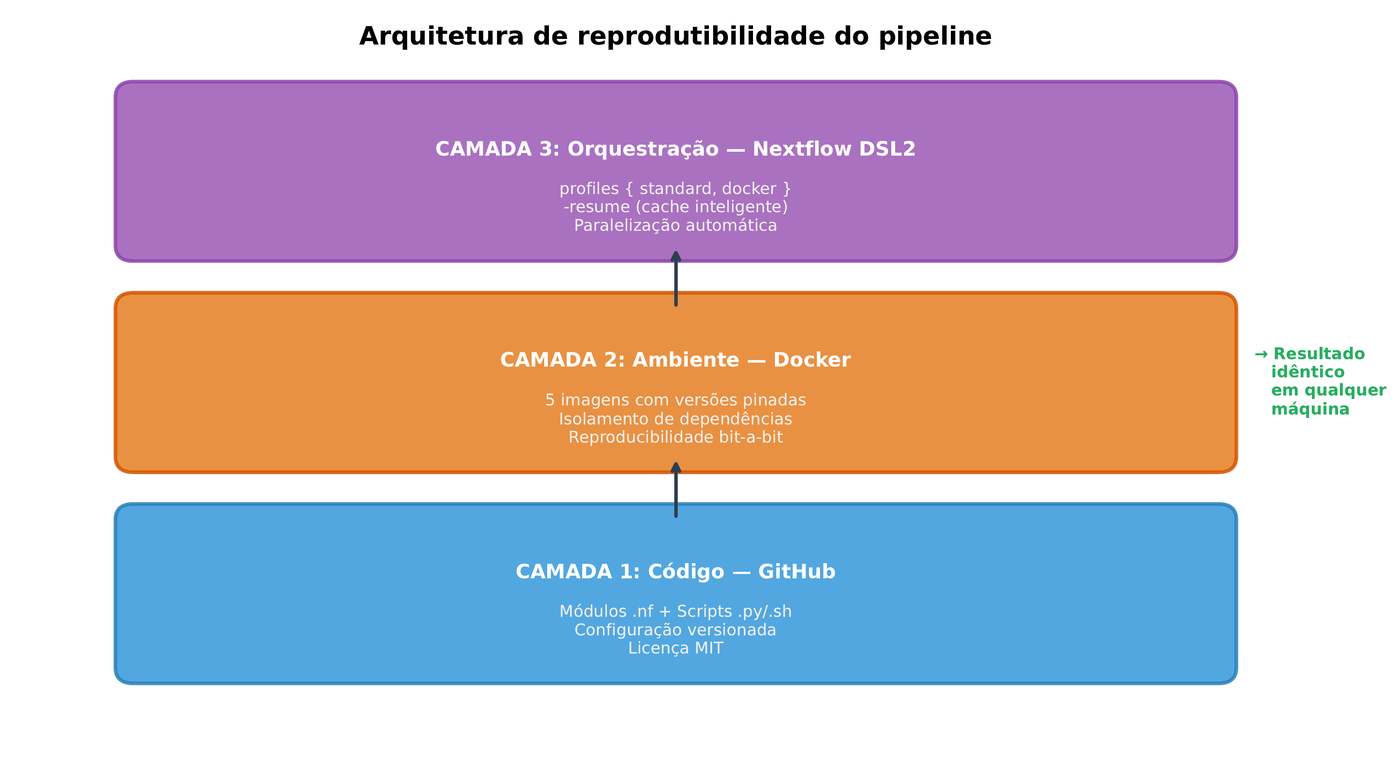
\includegraphics[width=0.85\textwidth]{imagens/camadas_reprodutibilidade.png}
    \caption{Três camadas de reprodutibilidade do pipeline: (1) código-fonte no GitHub, (2) ambiente isolado via Docker com versões pinadas, (3) orquestração via Nextflow DSL2.}
    \label{fig:camadas_reprodutibilidade}
\end{figure}
